%% 
%% Copyright 2007, 2008, 2009 Elsevier Ltd
%% 
%% This file is part of the 'Elsarticle Bundle'.
%% ---------------------------------------------
%% 
%% It may be distributed under the conditions of the LaTeX Project Public
%% License, either version 1.2 of this license or (at your option) any
%% later version.  The latest version of this license is in
%%    http://www.latex-project.org/lppl.txt
%% and version 1.2 or later is part of all distributions of LaTeX
%% version 1999/12/01 or later.
%% 
%% The list of all files belonging to the 'Elsarticle Bundle' is
%% given in the file `manifest.txt'.
%% 
%% Template article for Elsevier's document class `elsarticle'
%% with harvard style bibliographic references
%% SP 2008/03/01

%\documentclass[preprint,12pt,authoryear]{elsarticle}

%% Use the option review to obtain double line spacing
%% \documentclass[authoryear,preprint,review,12pt]{elsarticle}

%% Use the options 1p,twocolumn; 3p; 3p,twocolumn; 5p; or 5p,twocolumn
%% for a journal layout:
%\documentclass[final,12pt,times,authoryear]{elsarticle}
\documentclass[final,12pt,times,twocolumn,authoryear]{elsarticle}
%% \documentclass[final,3p,times,authoryear]{elsarticle}
%% \documentclass[final,3p,times,twocolumn,authoryear]{elsarticle}
%% \documentclass[final,5p,times,authoryear]{elsarticle}
%% \documentclass[final,5p,times,twocolumn,authoryear]{elsarticle}

%% For including figures, graphicx.sty has been loaded in
%% elsarticle.cls. If you prefer to use the old commands
%% please give \usepackage{epsfig}

%% The amssymb package provides various useful mathematical symbols
\usepackage{amssymb}
%% The amsthm package provides extended theorem environments
%% \usepackage{amsthm}

%% The lineno packages adds line numbers. Start line numbering with
%% \begin{linenumbers}, end it with \end{linenumbers}. Or switch it on
%% for the whole article with \linenumbers.
%% \usepackage{lineno}
\usepackage[utf8]{inputenc}
\usepackage[english]{babel} % English language/hyphenation
\usepackage[margin=1in]{geometry}
\usepackage{booktabs}
\usepackage{url}
\usepackage[hidelinks]{hyperref}
\usepackage{gensymb}

\hypersetup
{
	pdfauthor={Arielle Woods, Júlio Caineta, Sam Mark},
	pdfsubject={GEOL 2469},
	pdftitle={On the relationship between topographic metrics and signatures of damage to urban infrastructure}
}

% remove preprint footer
\makeatletter
\def\ps@pprintTitle{%
	\let\@oddhead\@empty
	\let\@evenhead\@empty
	\def\@oddfoot{\centerline{\thepage}}%
	\let\@evenfoot\@oddfoot}
\makeatother

\journal{GEOL2469 — Topographic Analysis}

\begin{document}

\begin{frontmatter}

%% Title, authors and addresses

%% use the tnoteref command within \title for footnotes;
%% use the tnotetext command for theassociated footnote;
%% use the fnref command within \author or \address for footnotes;
%% use the fntext command for theassociated footnote;
%% use the corref command within \author for corresponding author footnotes;
%% use the cortext command for theassociated footnote;
%% use the ead command for the email address,
%% and the form \ead[url] for the home page:
%% \title{Title\tnoteref{label1}}
%% \tnotetext[label1]{}
%% \author{Name\corref{cor1}\fnref{label2}}
%% \ead{email address}
%% \ead[url]{home page}
%% \fntext[label2]{}
%% \cortext[cor1]{}
%% \address{Address\fnref{label3}}
%% \fntext[label3]{}

\title{On the relationship between topographic metrics and signatures of damage to urban infrastructure}

%% use optional labels to link authors explicitly to addresses:
%% \author[label1,label2]{}
%% \address[label1]{}
%% \address[label2]{}

\author[geol]{Arielle Woods}
\ead{arielle.woods@pitt.edu}
\author[cmsp,geol]{Júlio Caineta}
\ead{julio.caineta@pitt.edu}
\author[geol]{Sam Mark}
\ead{szm18@pitt.edu}

\address[geol]{Department of Geology and Environmental Science, University of Pittsburgh, Pittsburgh PA, 15260, USA}
\address[cmsp]{Computational Modeling and Simulation, University of Pittsburgh, Pittsburgh PA 15260, USA}

\begin{abstract}
%% Text of abstract
We examined the influence of various topographic parameters on damage to infrastructure in Pittsburgh, Pennsylvania. Eight three-by-three block areas, selected to isolate variations in slope, drainage density, and drainage area, were chosen for field analyses. Investigators measured sidewalk cracks, tilted walls, and other common damaged features prevalent at all locations. Our statistical analyses suggest qualitative estimations of damage magnitude and structure age may be inconsistent between groups, which complicate an accurate interpretation of data. Additionally, we suggest that socioeconomic factors may control the distribution and severity of damaged infrastructure, as it is linked to older and less maintained infrastructure. Condition-desirability-utility (CDU) score, a qualitative metric provided for properties by Allegheny County, may be the best existing metric to capture these variations on a city-wide scale. Preliminary results suggest that slope and drainage density are positively related with damage and should be analyzed in further studies.

\end{abstract}

\begin{keyword}
%% keywords here, in the form: keyword \sep keyword
topographic metrics \sep human infrastructure  \sep damage
%% PACS codes here, in the form: \PACS code \sep code

%% MSC codes here, in the form: \MSC code \sep code
%% or \MSC[2008] code \sep code (2000 is the default)

\end{keyword}

\end{frontmatter}

%% \linenumbers

%% main text
\section{Introduction}
\label{s:intro}

The safety and stability of human infrastructure have been linked to different natural hazards such as landslides \citep{Polemio1999,Whitehead2009a,VonRuette2011} and floods \citep{Skilodimou2003,Arnaud-Fassetta2005,Youssef2011}, which are then linked to topography. Slope, drainage area, drainage density, and other topographic parameters influence landscape stability and hydrological dynamics, thereby threatening vulnerable aspects of human development \citep{Istanbulluoglu2005,Arnaud-Fassetta2005,Whitehead2009a}. Additionally, non-topographic parameters such as vegetated area, impervious surface area, and age of infrastructure can be controlling factors in how human infrastructure becomes damaged over time. In order to preserve existing infrastructure, and to safely and efficiently develop new and necessary housing units, roads, and electrical utilities, an improved understanding of how different geographic, geologic, and geomorphic trends influence different types of human infrastructure is necessary.

Pittsburgh, Pennsylvania has undergone numerous demographic, developmental, and economic shifts over the past 150 years. Infrastructure initially built in order to serve a burgeoning steel industry fell into disrepair during the 1980s as the area underwent a profound economic depression. Today, emergent local industries such as software development, medical technologies, and education necessitate shifts in local infrastructure \citep{Andes2017}. Additionally, the unique geographic setting of the city, nestled on steep hillslopes between the Monongahela, Allegheny, and Ohio Rivers, pose challenges for developing structurally sound roads, homes, and sewer systems \citep{Hopkins2014}.

In this analysis, we focus on isolating topographic parameters measurable from 30 meter resolution Digital Elevation Models (DEMs) and use field observation to examine their individual influence on damaged human infrastructure. This research group focused on the influence of drainage density, while other collaborators examined slope and drainage area, all contributing to the same dataset. We hypothesize that increased drainage density, increased drainage area, and increased slope will all lead to a greater degree of damaged infrastructure when normalized to account for variations in influential non-topographic metrics. By better constraining the relationships between different aspects of regional topography and different aspects of human development, we hope to contribute to an improved framework of how to sustainably create new infrastructure as the region continues to change. 


\section{Methodology}
\label{s:methods}

\subsection{Site selection}
We used a 30 meter resolution DEM provided by Allegheny County to isolate areas in which drainage density (DD) differed substantially but slope (S), drainage area (DA), and wetness index (WI) remained relatively constant. Additionally, we attempted to control for the potentially influential non-topographic metrics of housing age (HA) and soil type (publicly provided by Allegheny County) and vegetative canopy and impervious cover (provided by the National Land Cover Database). A more comprehensive review of our site selection methodology can be found in our previous submission (HA5, 11/8/17). 

\subsection{Field data collection}
Two sites were selected for analysis (\autoref{fig:map}). The high (subscript H) and low (subscript L) DD sites, centered at approximately $40\degree28'18.14$ N $80\degree00'44.52$ W and $40\degree28'06.58$ N $80\degree01'15.52$ W, respectively, where each span approximately three city blocks of the city’s more sparsely populated north side. We collected 57 data points corresponding to damaged infrastructure on 11/19/2017, primarily focusing on types of damage such as cracked sidewalks and tilted house walls, which would likely be prevalent at all of the sites to allow for a more in depth comparison. The other three research groups collected data in a similar manner, contributing to a total of 183 data points collected in 8 neighborhoods, each approximately three blocks by three blocks, in Pittsburgh. Each research group isolated a topographic metric and collected field data in an area related to a high value of that topographic metric and another area related with a low value. The three other groups selected DA and S (two groups) as the isolated topographic metrics.

\subsection{Statistical analysis}
The statistical analysis of the collected data points focused on both aggregate data of all sites, as well as the individual influence of specific topographic metrics on damaged infrastructure. Topographic metrics include those derived from the DEM, as well as the local slope measured while surveying. For the purpose of aggregate statistics, we grouped the study sites that selected slope as the isolated metric, combining the corresponding high and low sites into single pairs.

We approached uncertainty assessment by comparing the qualitative and subjective metrics of damage, such as the damage magnitude and the apparent age of structure, with quantitative metrics, such as length and tilt. In particular, we also sought to investigate how the research groups evaluated the qualitative measures differently.

In this study, we gave more emphasis to simple univariate and bivariate statistics, followed by the visualization of the accurate distribution of the data given by histograms, as well as scatter plots. All statistical analyses and derived plots were performed in MATLAB.\footnote{The code used to conduct these experiments is publicly available at \url{https://github.com/iled/topodamage}.} It requires MATLAB version R2016b or higher, with the Mapping Toolbox and the Statistics and Machine Learning Toolbox enabled, along with the third party TopoToolbox installed.


\section{Results}
\label{s:results}

Initial aggregate analyses of data points from all study sites suggest sidewalk and walls compose the majority of total damaged points (\autoref{fig:histtype}). In particular, walls were the most common identified structure in both DD sites, whereas for the others it was sidewalks (Table 1). For all groups, average magnitude of damage is greater at high site types than low site types (\autoref{t:strutmode}). \autoref{t:sitemag} shows that damage of greater magnitude (at least 3) was assigned more frequently to the sites of higher DD (29.5\%) and higher S (27.3\%).

\begin{table}[]
	\centering
	\caption{Most frequent structure (mode) and average damage magnitude per site type.}
	\label{t:strutmode}
	\begin{tabular}{@{}cccc@{}}
		\toprule
		Site type & Count & Structure & Magnitude \\ \midrule
		DD\_L     & 26    & 4              & 1.81           \\
		DD\_H     & 27    & 4              & 2.52           \\
		DA\_L     & 20    & 1              & 1.30           \\
		DA\_H     & 30    & 1              & 2.07           \\
		S\_H      & 45    & 1              & 1.96           \\
		S\_L      & 39    & 1              & 1.23           \\ \bottomrule
	\end{tabular}
\end{table}

We then attempted to find evidence of a relationship between the topographic metrics as measured from the DEM and the damage magnitude (see \autoref{fig:topodmgsww} in the \autoref{s:sm}). No discernible connection was clear. Because sidewalks and walls were the most commonly measured structures in the collective survey, a similar approach was used with the corresponding quantitative damage metrics, length and tilt (\autoref{fig:topotiltlen}). Here, length refers to the extension of cracks, including all types of structure that admit such type of damage (walls, sidewalks, roads), and tilt to an angular displacement from the vertical (walls, fences, poles).

\begin{table}[]
	\centering
	\caption{Distribution of damage magnitude values per site type.}
	\label{t:sitemag}
	\begin{tabular}{@{}ccccccc@{}}
		\toprule
		Site type \textbackslash\, Magnitude & 1  & 2 & 3 & 4 & 5 & \textgreater= 3 \\ \midrule
		DD\_L                              & 16 & 3 & 3 & 4 & 0 & 15.9\%          \\
		DD\_H                              & 7  & 7 & 7 & 4 & 2 & 29.5\%          \\
		DA\_L                              & 15 & 4 & 1 & 0 & 0 & \, 2.3\%           \\
		DA\_H                              & 14 & 7 & 4 & 3 & 2 & 20.5\%          \\
		S\_H                               & 24 & 9 & 5 & 4 & 3 & 27.3\%          \\
		S\_L                               & 33 & 4 & 1 & 1 & 0 & \, 4.5\%           \\ \bottomrule
	\end{tabular}
\end{table}

To further constrain this analysis, and in compliance with the first result, DD and S would be the two variables to look in more depth. However, there were only a limited number of points where DD values were available. Accordingly, \autoref{fig:slopetiltlen} compares the values of regional (DEM-derived) and local (field measured) slope against length and tilt. In this figure, only the sites that isolated slope are included, since the others purportedly fixed that metric within a certain range. The first observation is that the high (blue) and low (green) sites are in agreement with the expected range of regional slope values. This separation is not equally strict for the local slope, which is not unexpected, since regional slope cannot capture all the variability that exists at a local scale, although in general regional and local slope tend to covary (see \autoref{fig:slopelocalreg}). Secondly, both regional and local slopes seem to have a higher number of points corresponding to higher values of tilt; such evidence is not noticeable for the length. This observation also supports the evidence that a higher slope has a positive relationship with damage in infrastructure, here verifiable in the form of angular displacement. It should be noted that a higher number of data points would help to attest this statement.

\begin{figure}[hbt]
	\centering
	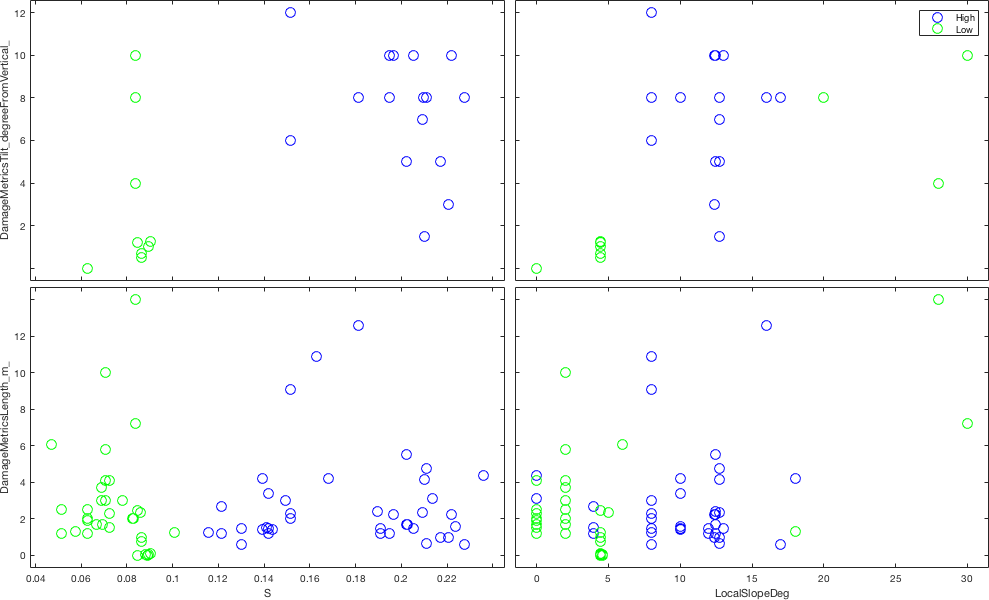
\includegraphics[width=\linewidth]{fig/tilt_and_length_vs_slope_site}
	\caption{Regional (left) and local (right) slope vs tilt (up) and length (bottom).}
	\label{fig:slopetiltlen}
\end{figure}

\section{Discussion}
\label{s:disc}

The relative abundance of higher magnitude damages in high drainage density and high slope sites seems to be a rough indicator of correlation between these metrics and damage degree (Table 1). However, more in depth examination of these data suggest the metric of magnitude may not reflect physical reality. Our statistical analysis of the aggregate data suggests the qualitative estimation of damage magnitude varies widely among sampling teams (\autoref{fig:histgroups}). Magnitude 1 was the most commonly assigned category, and all groups were conservative in assigning higher magnitude values to their measurements. The distribution of magnitudes was quite variable among groups; the relatively even distribution in the Buford group data is contrasted by the CFW group assigning magnitude 3 only once, and never making use of magnitudes 4 or 5. Further illustrating the flawed data collection procedure is that magnitude appears to be unrelated to the quantitative methods of assessing degree of damage, such as crack length and degree of tilt (\autoref{fig:qualquant}). The statistical distribution for tilt and magnitude appear to be inversely related for the Buford and CFW groups, rendering this portion of the data contradictory (\autopageref{fig:histgroups}).

\begin{figure}[hbt]
	\centering
	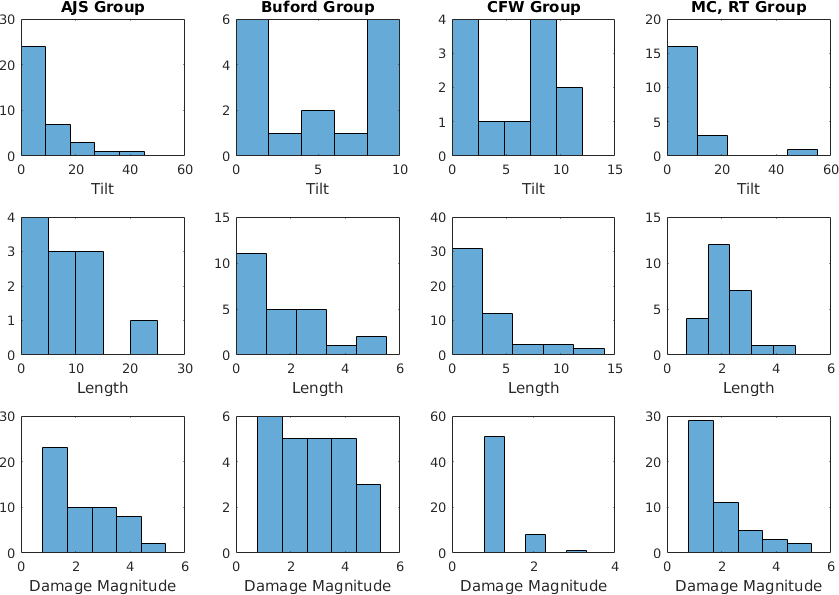
\includegraphics[width=\linewidth]{fig/hist9-9}
	\caption{Distribution of values for the quantitative (tilt and length) and qualitative metrics of damage per each group.}
	\label{fig:histgroups}
\end{figure}

\begin{figure}[hbt]
	\centering
	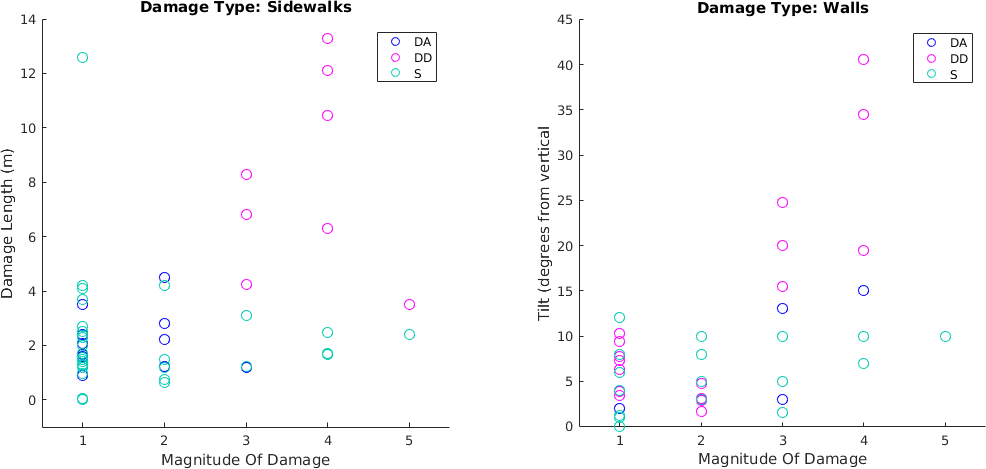
\includegraphics[width=\linewidth]{fig/Actual_v_MagDam}
	\caption{Qualitative (magnitude) vs quantitative (length and tilt) metrics of damage for sidewalks and walls.}
	\label{fig:qualquant}
\end{figure}

Controlling for structure type by looking at only sidewalks or only walls, it is apparent that the expected positive relationship between measured damage and perceived magnitude is absent for the DA and S sites; the DD site appears to have more realistic magnitudes assigned to sidewalk crack length and wall tilt, although this is represented by a small number of data points (\autoref{fig:qualquant}). The range of measured values for tilt and length is also highly variable among groups, and without confirmation that these discrepancies would be agreed upon by all groups, these apparent perceptional biases preclude confident intercomparison. Such inconsistencies make it difficult to compare or combine group data, and to draw meaningful conclusions about the broader influence of topography on damage. These discrepancies bear implications for future studies; workers should attempt to homogenize their evaluations before field analyses take place in order to more accurately compare qualitative values between sites.




\subsection{Additional metrics and sources of damage}

While age of housing may exert some control on damaged infrastructure, our qualitative assessment and contact with residents suggest property value may be a more significant factor. Our high drainage density site contained numerous abandoned homes and other infrastructure largely left to disrepair. One resident, noticing our interest in a large sidewalk crack which potentially represents a public safety hazard, mentioned that she had brought the issue to the attention of the city several times in the past five years and that nothing had been done to remediate it. This suggests a combination of socioeconomic factors not captured by our age of housing metric control infrastructure deformation and damage. Condition-desirability-utility score, a holistic metric used to evaluate property value, may best capture these shifts across different areas. This categorical evaluation ranges from 8 (very good) to 0 (unusable). A comparison of CDU score and quantitative damage severity (crack length and wall tilt degree) shows that greater degrees of damage occur in areas with lower CDU score (\autoref{fig:cduvert}).

\begin{figure}[hbt]
	\centering
	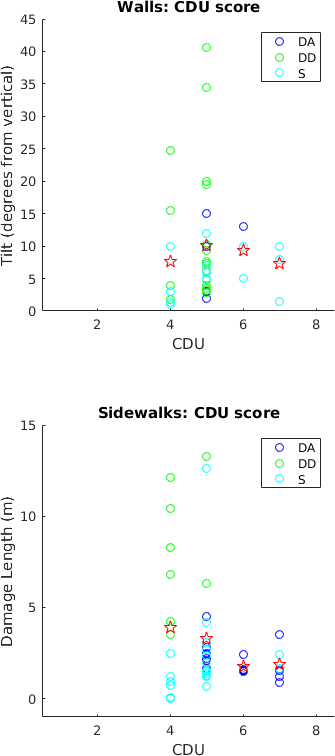
\includegraphics[width=\linewidth]{fig/CDUverticalplot}
	\caption{CDU vs tilt and length for walls and sidewalks.}
	\label{fig:cduvert}
\end{figure}

\section{Conclusions}
\label{s:conc}

Based on the findings of this studies, we offer few concrete conclusions regarding the association between landscape and human infrastructure, but some potentially instructive guidelines for future research in this area. We provide limited evidence that a positive relationship exists between areas of high DD and areas of high slope. More specifically, we show that there seems to exist a link between local slope and angular displacement of structures akin to such type of damage, like walls, fences and poles. We argue that insufficient evidence was apparent for a relationship between slope, drainage density, and drainage area and magnitude of damage.

Additionally, we suggest that socioeconomic factors between neighborhoods may be responsible for a significant portion of damaged infrastructure. We propose CDU score as a metric that may be used as a proxy for the combination of non-topographic qualitative factors which lead to certain neighborhoods falling into physical disrepair.

The statistics used in this study, although basic, were preferred for their clearer interpretation. By analyzing the efficacy and consistency of our sampling methods, we attempt to address the gap of uncertainty assessment, thus contributing to a framework for future research. Once data collection procedures and evaluation criteria are homogenized, more complex statistical analyses can be applied in order to more precisely assess the link between topography and damage to human infrastructure. 


%% The Appendices part is started with the command \appendix;
%% appendix sections are then done as normal sections
%% \appendix

%% \section{}
%% \label{}

%% If you have bibdatabase file and want bibtex to generate the
%% bibitems, please use
%%
\bibliographystyle{elsarticle-harv} 
\bibliography{topodamage}

%% else use the following coding to input the bibitems directly in the
%% TeX file.

%% \begin{thebibliography}{00}

%% \bibitem[Author(year)]{label}
%% Text of bibliographic item

%% \bibitem[ ()]{}

%% \end{thebibliography}

\newpage

\appendix

\onecolumn

\renewcommand\thefigure{SM.\arabic{figure}}    
\setcounter{figure}{0}    

\section*{Supplementary material}
\label{s:sm}

\begin{figure}[hbt]
	\centering
	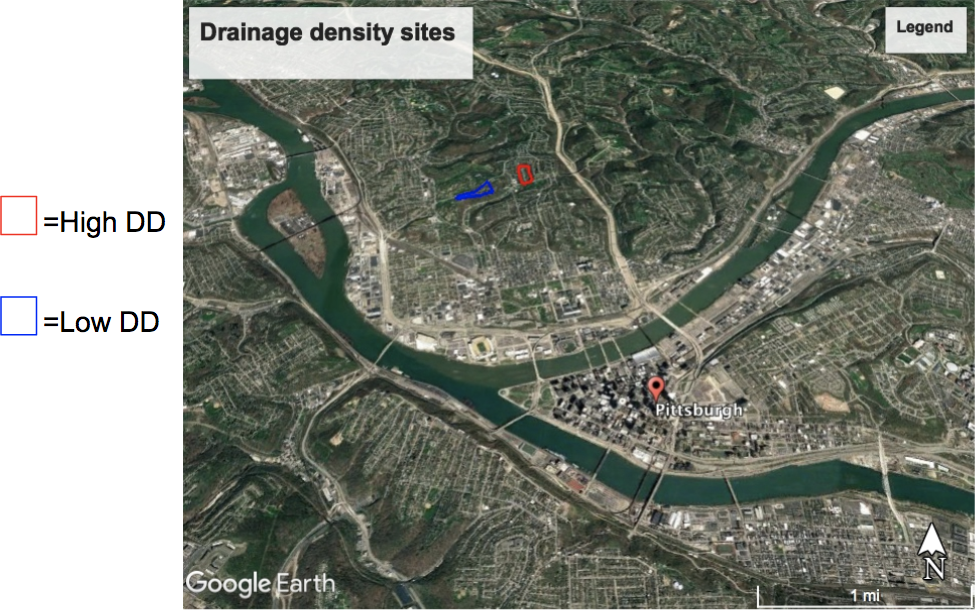
\includegraphics[width=\linewidth]{fig/ddmap}
	\caption{Location of the drainage density sites in Pittsburgh.}
	\label{fig:map}
\end{figure}

\begin{figure}[hbt]
	\centering
	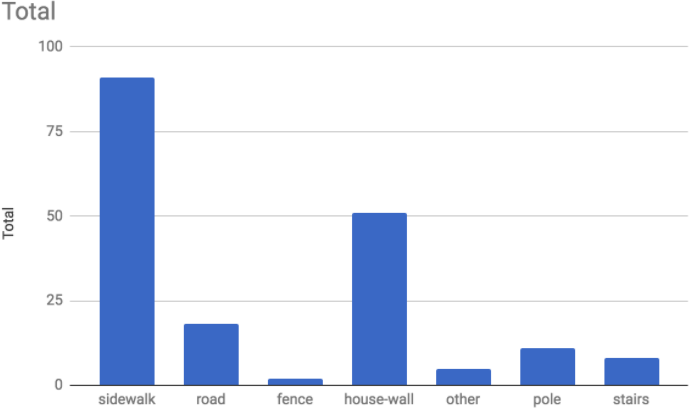
\includegraphics[width=\linewidth]{fig/aggregatedamagetype}
	\caption{Frequency of each type of structure.}
	\label{fig:histtype}
\end{figure}

\begin{figure}[hbt]
	\centering
	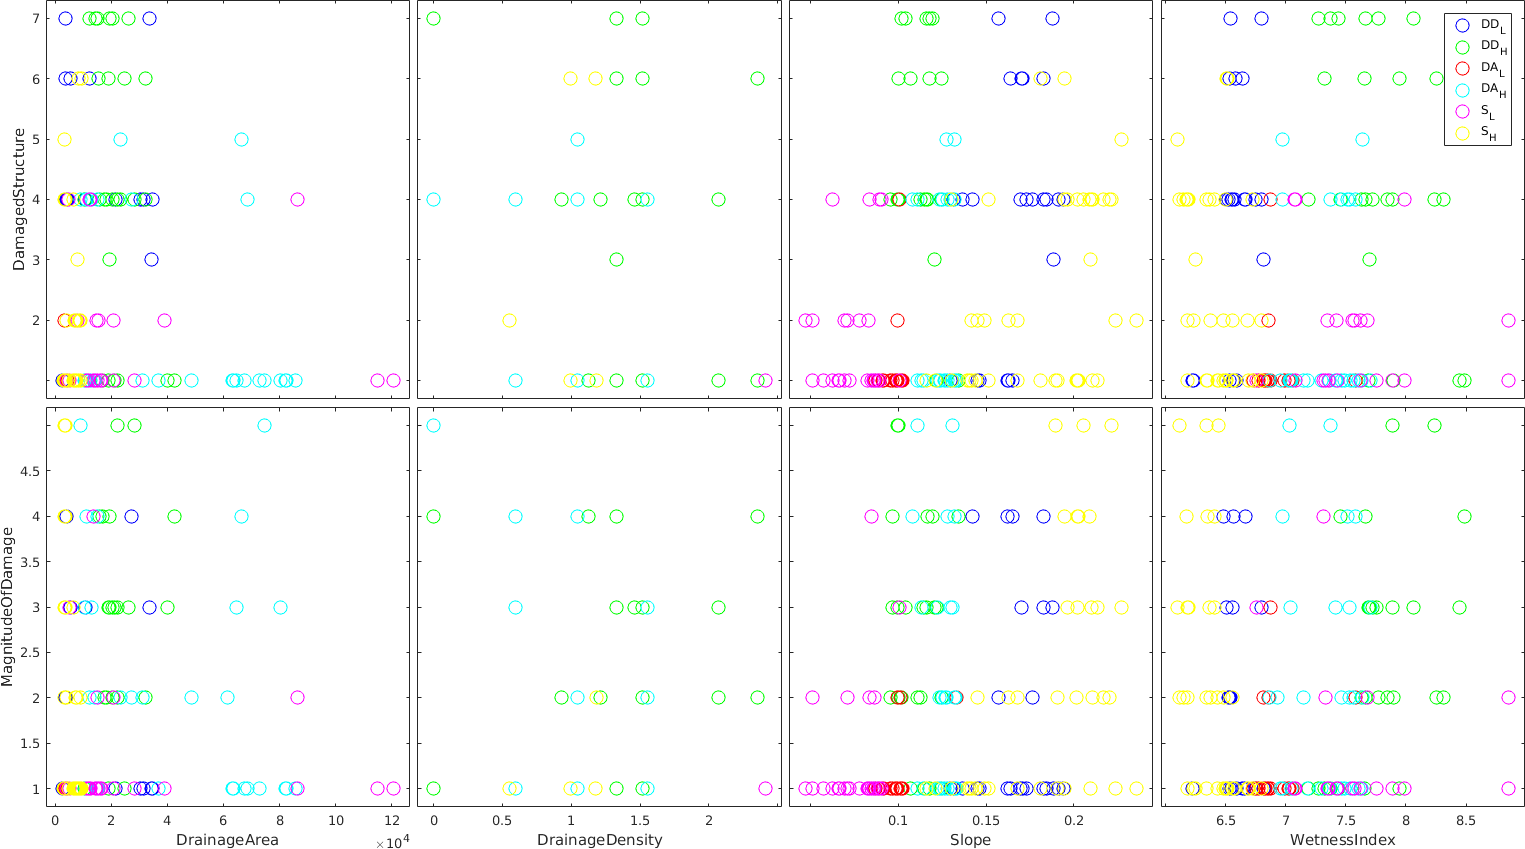
\includegraphics[width=\linewidth]{fig/topomaps_vs_damagemag_strut}
	\caption{Topographic metrics vs damage magnitude for each type of structure (1: sidewalk, 2: road, 3: fence, 4: house-wall, 5: other, 6: pole, 7: stairs).}
	\label{fig:topodmgsww}
\end{figure}

\begin{figure}[hbt]
	\centering
	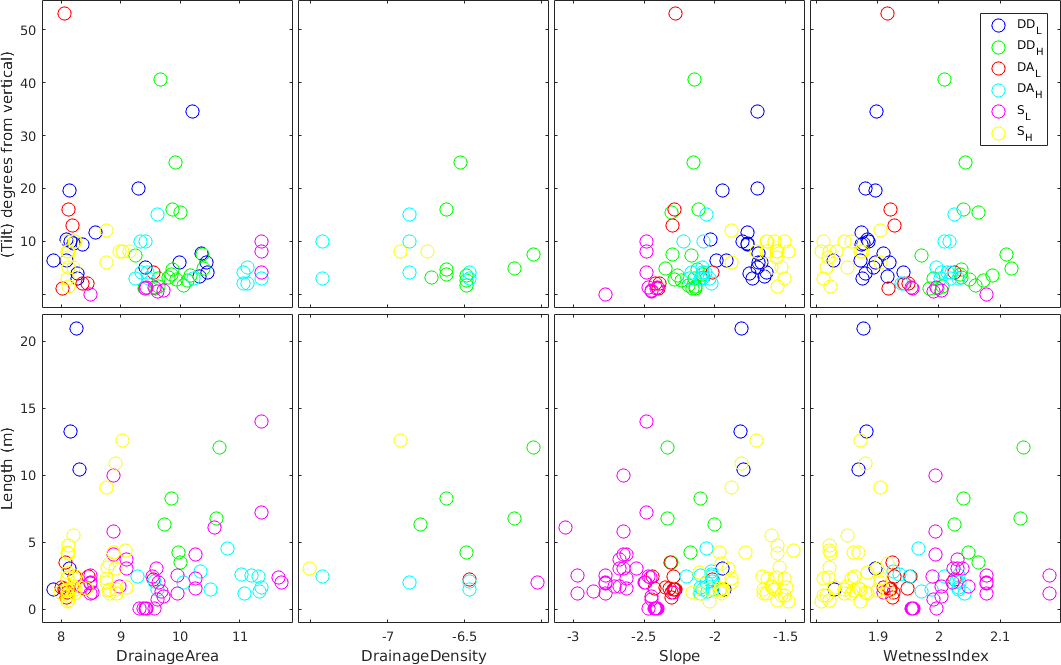
\includegraphics[width=\linewidth]{fig/plotmatrix_topo_vs_tilt_length_all_sites}
	\caption{Topographic metrics vs tilt and length.}
	\label{fig:topotiltlen}
\end{figure}

\begin{figure}[hbt]
	\centering
	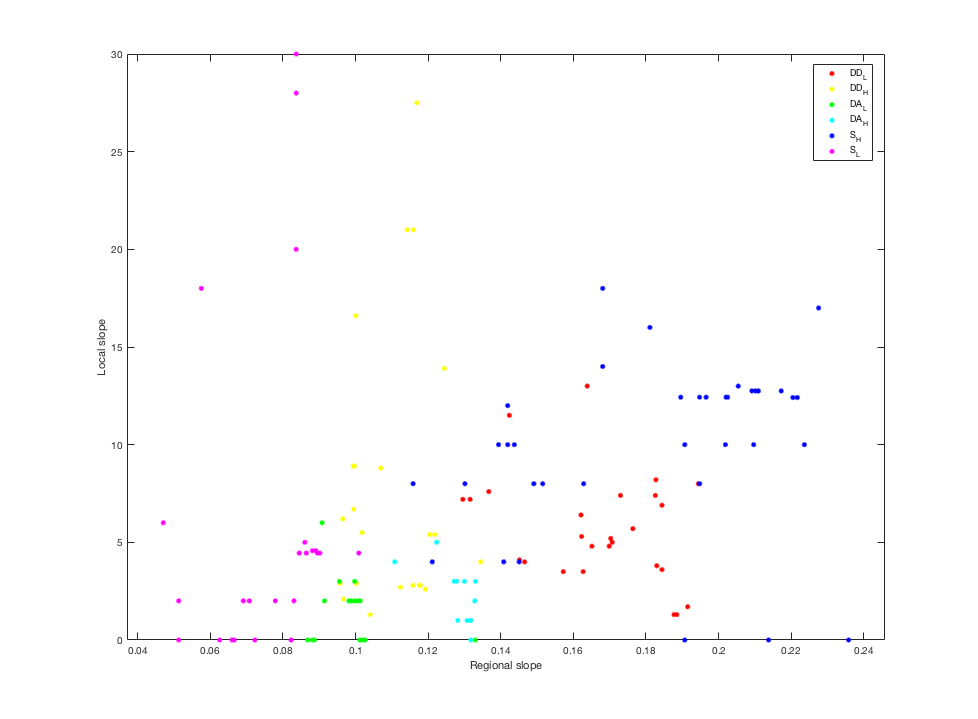
\includegraphics[width=\linewidth]{fig/local_vs_regional_slope_all_sites}
	\caption{Local vs regional slope for all sites.}
	\label{fig:slopelocalreg}
\end{figure}

\begin{figure}[hbt]
	\centering
	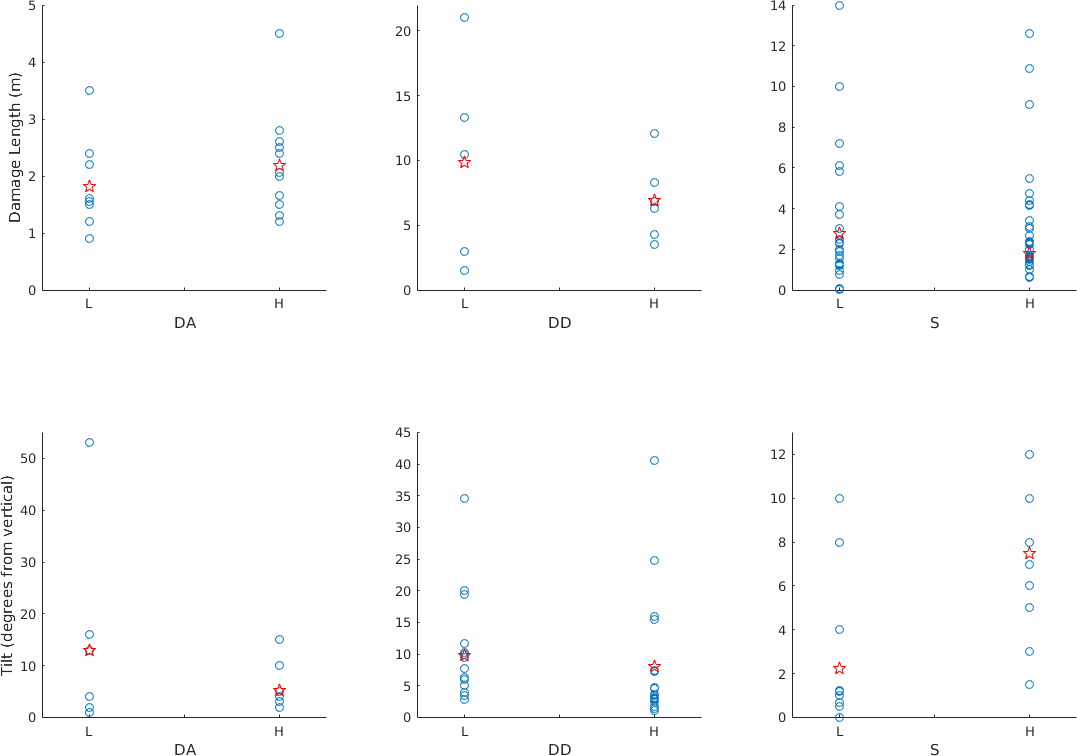
\includegraphics[width=\linewidth]{fig/length-tilt-LH}
	\caption{Distribution and means (red star) of damage for paired study sites: measured length (top row) and tilt (bottom row) of damaged features.}
	\label{fig:distmeansdmg}
\end{figure}

\begin{figure}[hbt]
	\centering
	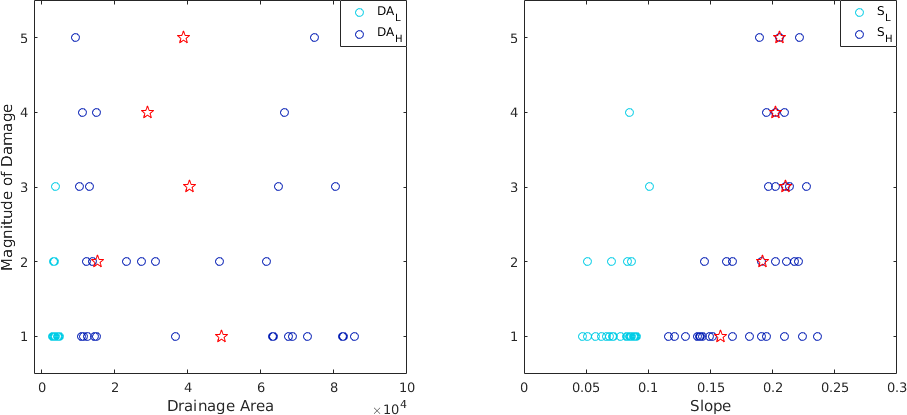
\includegraphics[width=\linewidth]{fig/Mag_DA_S_redstart}
	\caption{Magnitude of damage compared to the interpolated topographic metric (pixel scale) for drainage area and slope group data. Drainage density is excluded because all DD-L points are \texttt{NaN}. Red stars indicate mean values for magnitude of damage category 1-5, for DA-H and S-H sites only (Low sites excluded due to more limited number of data points).}
	\label{fig:maginterp}
\end{figure}

\begin{figure}[hbt]
	\centering
	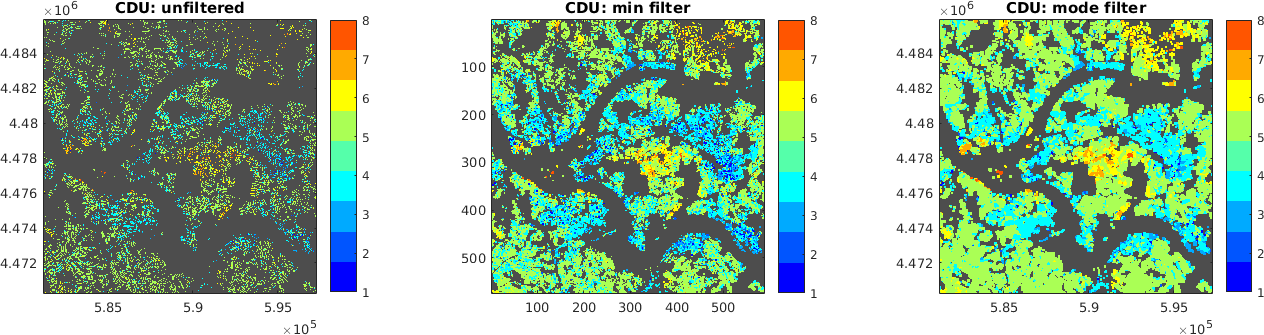
\includegraphics[width=\linewidth]{fig/CDUfiltercompare}
	\caption{Comparison of the generated maps for CDU: original, without resampling (left); resampled with a minimum filter (center); resampled with a mode filter (right).}
	\label{fig:cducompare}
\end{figure}

\end{document}

\endinput
%%
%% End of file `elsarticle-template-harv.tex'.
